\chapter{Territorial swarming}
\label{chap:myModel}
When the simulation starts the UAVs begin searching the world for targets.  While scanning the world they update their internal belief model.  This internal model is shared with other members of the swarm when they are within communication's range of each other.  This model contains data regarding each UAV's confidence that a geographic region is clear and a list of known targets.  Section~\ref{sec:uavBelief} describes this model in detail.

When a target is found the UAV assigns an initial task status to the target and announces the discovery of the target.  The original UAV and anyone within communication's range compute a scoring value to determine who is the most appropriate UAV to monitor or attack the target.  Soon after the other UAVs in range who heard the initial target announcement will re-broadcast their internal belief models, and therefore propagate the target discovery throughout the swarm.

\section{UAV Communications}
While each agent within the swarm is capable of self actualization, mission performance improves when the agents work as a team.  To work as a team the UAVs must communicate with each other.  The simulation done in this work limits the communication range of UAV's to a percentage of the maximum world distance.  Given that the mission occurs in a square or rectangular environment, the maximum world distance occurs between opposite corners along a diagonal that bisects the mission area.  %By specifying the communication range as a percentage of the world size the algorithms in this work are invariant of the physical world's size.

From a communication perspective the swarm can be thought of as a mobile ad hoc network (sometimes referred to as a MANET).  This is because the network connections among the UAVs is dynamic and unpredictable.  There are no designated network control nodes.  Every UAV is equally likely to broadcast spontaneously.  A simple approach to make sure all agents within the swarm receive all communications is to ``flood'' the broadcasts.  When an agent hears a particular message for the first time it is required to rebroadcast the message.  The advantage to this simple approach is that it requires no coordination or management overhead for communications support within the swarm.

While simple to implement this flooding approach has many drawbacks.  Many neighboring UAVs will likely have already heard the message themselves from the original source meaning there are redundant broadcasts.  Many neighboring UAVs will hear the message simultaneously and will jam each other when they all attempt to rebroadcast the message.  When the message collisions occur the data transmissions will be garbled forcing a re-transmission that further adds to the network congestion.  This is known as the broadcast storm problem as originally put forth by~\cite{bstorm}.

Finding ways to optimize MANETs and to eliminate the broadcast swarm problem is a whole field of research unto itself.  The research performed in~\cite{epidemicManets} and ~\cite{analysisOptNodeDen} are relevant to UAV swarms in that they find ways to minimize the number of needed transmissions and ways to reduce transmission power levels.  The standard approach is to not always rebroadcast a message when it is first heard and instead only rebroadcast based on chance.  This is known as the Probabilistic Flooding technique.  There are many variants to this technique with some described in~\cite{probFloodVariants}.  For our purposes the version described in~\cite{simpleProbFlood} was used.  In this case the probability that a UAV will rebroadcast any individual message is computed by equation~\ref{eq:probFlood} where $hop$ is the number of times the message has already been rebroadcasted and $num\_uavs$ is the number of UAVs in the swarm.  This equation states that when a message is first generated it is very likely it will be rebroadcasted but each subsequent broadcast becomes less likely to occur.

\textbf{I would be useful to summarize any results from Jiang that would indicate that this is a good strategy and how well it performed. Also this whole discussion about MANETS assume that there is connectivity throughout the network. This will mean that eventually all UAVs should hear all broadcasts. It also means that if a UAV or group of UAVs is totally isolated from the rest of the swarm that any information it (or they) broadcast is lost to the rest of the swarm. This appears the case in Figure 7-1 later where most of the UAVs are isolated from each other. The impact this has on performance is an important aspect of this approach and I would think you should complete the discussion here about how communication works in those cases.	What happens when you hear old news (i.e. a rebroadcast over multiple hops that arrives so late you’ve already heard a more recent version of that message from the sender)?}

\begin{equation}
\label{eq:probFlood}
P(rebroadcast) = 1 - \frac{hop}{num\_uavs - 1}
\end{equation}

\section{UAV Tasks}
UAV's compete to selectively perform tasks in order to complete the mission.  The available tasks are \textit{Search}, \textit{Monitor}, and \textit{Attack}.  The Search task is always available for all UAVs to carry out.  The Monitor and Attack tasks can only be executed in association with a suspected or confirmed target respectively.  UAVs may only perform a single task at a time therefore no UAV may \textit{Monitor} and \textit{Attack} simultaneously.

\subsection{Search}
No target locations within the simulated world are known \textit{a priori}.  The UAV's must discover all targets individually.  The goal of searching is for the swarm to map out the locations of targets and maintain a roving surveillance presence. In formal terms Search is guided by the confidence or certainty of the swarm that a location contains or does not contain targets.  Over time this certainty erodes in locations that are not being actively watched.  UAVs that are performing Search will attempt to maximize their certainty of the world by scanning the most uncertain or least confident locations.  Uncertainty is defined in detail in chapter~\ref{sec:uavBelief}.

A search-and-track survey paper by ~\cite{senanayake} highlights many search algorithms to choose from. Our search was accomplished by mimicking the foraging behaviors of animals with an algorithm similar in principle to a \textit{L\'evy Flight} (\cite{humphries}) but adapted to a discrete world instead of a continuous world.  The L\'evy Flight algorithm is a type of biased random walk.  The UAV foraging algorithm is enumerated in algorithm~\ref{alg:forage} in appendix~\ref{sec:algorithms}.  The algorithm will randomly select a grid cell within the world or it will divide the world into kernels, compute the uncertainty of each kernel, and randomly select a cell within the most uncertain kernel.  The kernel size must divide equally into the number of rows and columns in the world.  The weighting between searching a kernel area versus random world locations is controlled by the $randomWeighting$ parameter in algorithm~\ref{alg:forage}.

The balance between local kernel searching and completely random locations is a function of UAV density (number of UAVs divided by world area) and their communication ranges.  Therefore this value will be unique to every swarm configuration.  Assuming adequate communication ranges the weighting between searching random locations and within kernels should be biased towards searching local kernels if the density of UAVs  in the swarm is high.  If the density is low then the weighting should be set closer to a half and half split.  With a high density of UAVs it is inefficient for UAVs to randomly jump from one end of the world area to the other.  Time is wasted since other UAVs are already covering the rest of the world and due to the UAV density belief data is able to propagate across the world.  With a low density swarm it is advantageous to bias towards random locations because it encourages the UAVs to wander about.  This allows UAVs to propagate data from one side of the world to the other by physically carrying it.  

%\textbf{TODO: IN reference to "within the most uncertain kernel"	This worries me. The mantra of swarming systems is to sense and act locally. Here you are sensing and acting globally since you take the most uncertain kernel. I can see two issues that I don’t know whether you address later:	If your communications range is short enough, I suspect you may not hear about distant UAV activities. Since the only way to reduce uncertainty in a cell is through UAV activity, the most uncertain cells will be those most distant from me that I haven’t heard anything about. I may then be inclined to select a move to a distant region only because I didn’t hear about the fact that they had already been searched. 	Since all UAVs are looking for the highest uncertainty kernel what is to prevent them from all selecting the same kernel to move towards leading to herding behavior? } 

%https://en.wikipedia.org/wiki/L%C3%A9vy_flight

Once a search cell has been selected the UAV will fly towards it until another task takes precedence or the uncertainty in the cell falls below a user configured threshold.  While performing the search task UAVs point their sensor payloads towards the selected search cell even if they are not within range.  While traversing the world the UAV will opportunistically scan all cells encompassed by the sensor's field of view.  The uncertainty of cells change when UAV sensors can cover it or when an update from another UAV in the swarm provides new data about the cell. When the uncertainty in the selected search cell drops below the user configured threshold then the UAV will select a new cell to investigate.  

If the UAV's own sensors causes the uncertainty of a cell to drop low enough (as opposed to an update from a fellow swarm member) then that UAV is likely to stay in the local kernel area.  This is because the UAV purposefully flew to this area since it was the most uncertain kernel.  Therefore it will likely scan the local cells in the kernel, at random, until the local kernel is no longer the most uncertain kernel.  An atypical case occurs when the UAV selects a completely random location in the world.

Since the search algorithm analyzes the global uncertainty to select the most uncertain kernel to go explore readers might assume that the swarm performs herding behaviors since all swarm members will fly to the same region.  If the swarm had a centralized data model that was shared amongst all members instantaneously this would be true.  Since it takes time for data to propagate across the swarm and members of the swarm do not fully trust one another each swarm member has a different definition of the most uncertain kernel.  This issue of trust is explain later in section~\ref{sec:mergingBeliefs}.

\subsection{Monitor}
The Monitor task requires a UAV to watch a potential target.  The UAV will point its sensing payloads at the target, confirm the target's identity, track the target, and perform a battle damage assessment after the target has been struck.  These steps are broken down into states within the Monitor task.  The monitor task state transitions are illustrated in figure~\ref{fig:monitor}.

\subsubsection{En Route}
When a UAV first starts the Monitor task it begins flying towards the target and points its payloads in the target's direction.  As the UAV flies it continues to scan any cell within its payload's field of view until the target is within range.  Once the target is in sensor range the UAV transitions to the Confirm state.  

When the UAV is in sensor range it will begin orbiting the target.  If the target moves more than some user configurable percentage of the sensor's range then the UAV will adjust its flight path and recenter the orbit over the target's new location.

\end{multicols*}

\begin{figure}[H]
	\centering
	%\includegraphics[width=\linewidth,height=\textheight]{imagefile}
	\includegraphics[scale=0.6]{uav_monitor_states.png}
	%	\includegraphics{uav_monitor_states.png}
	\caption{Monitor sub-states}
	\label{fig:monitor}
\end{figure}

\begin{multicols*}{2}

\subsubsection{Confirm}
When the target is within sensor range the UAV will focus its sensors on the target.  This causes the sensors to stop performing a wide area scan and to zoom in on the target's suspected world cell location.  At this time the UAV is analyzing the sensor data to determine if the suspected target is a real target or if it's a false positive and no target exists.  No other targets can be detected during this focused scan and the certainty of any cells that happen to be in the field of view do not change.  If the suspected target is fake then the UAV exits the Monitor task.  If the target is confirmed to be real then the UAV transitions to the Track Target state.  For purposes of this experiment the target confirmation analysis process was assumed to take 10 seconds.  No attempt was made to model real world physics of target identification from raw sensor data.

\subsubsection{Track Target}
In this state the UAV is continuing to point its payloads at the target but the sensors have resumed a wide area scan in hopes of finding other nearby targets.  The UAV stays in this state until the target outruns the UAV's sensors and is lost, the target is struck by a weapon, or a user configurable timeout occurs.  When the UAV first enters this state it requests a weapon's strike on the target from the swarm.  The details of the weapon's strike request are presented in chapter~\ref{sec:uavBelief}.  The timeout is useful in the cases where all nearby UAVs are busy performing other high priority tasks or are also stuck waiting for a weapon strike.  This timeout acts as a tie breaker to prevent everyone waiting for a strike simultaneously.  The downside is that the target is briefly ignored when the timeout engages.

\subsubsection{Battle Damage Assessment}
When the monitoring UAV detects a weapon's strike on the target it will transition from wide area scan tracking to narrow focused scans of the target's location.  As in the Confirm state during this focused scan no other targets can be detected and the certainty any cells that happen to be in the field of view do not change.  This state represents the time it takes for the UAV to analyze its sensor data to determine if the target was destroyed or if it is still active.  Again, for purposes of the experiment it was assumed that battle damage assessment (BDA) takes 10 seconds to complete.  No attempt was made to model real world physics of target status from raw sensor data.

If the target is still active after the weapon's strike the UAV will transition back to the Track Target state and request another strike from the swarm.  If the target was destroyed then the UAV will exit the Monitor task.


\subsection{Attack}
The Attack task mechanics are similar to the Monitor task in that the UAV will fly towards the target and point all of its sensors at the target.  The UAV will plot a course such that its heading is aligned with the best attack angle relative to the heading of the target.  The UAV will re-plot a new course if the target moves a significant distance.  This distance is user configurable.  The UAV will wait until the distance to the target is below some percentage of the weapon's max range before firing.  For purposes of this experiment the percentage was set to 80\%.  An activity diagram describing the process is shown in figure~\ref{fig:uavAttackActivity}.  In parallel to the actions shown in the diagram the UAV is constantly flying along the last computed Dubin's Path.

The weapon time-of-flight is not modeled.  Weapon strikes are considered instantaneous.  When the weapon is deployed the UAV has completed the task.  The UAV may assign itself a new task and begin maneuvering to a new destination.  However, the UAV performing the Monitor task may request another weapon strike from the swarm if the target was not destroyed.  Therefore the UAV that completed the Attack task might decide to perform the Attack task again since it's likely the closest strike platform available.  The details of this process are explained in chapter~\ref{sec:uavBelief}.  A summary of the interactions between the monitor and attack roles can be seen in figure~\ref{fig:monitorAttacKSequence}.

\end{multicols*}

\begin{figure}[H]
	\centering
	%\includegraphics[width=\linewidth,height=\textheight]{imagefile}
	\includegraphics[scale=0.75]{uav_activity_attack.png}
	\caption{UAV Attack Activity}
	\label{fig:uavAttackActivity}
\end{figure}

\begin{figure}[H]
	\centering
	%\includegraphics[width=\linewidth,height=\textheight]{imagefile}
	\includegraphics[scale=0.75]{monitor_attack_sequence.png}
	\caption{Monitor and Attack Sequence Interactions}
	\label{fig:monitorAttacKSequence}
\end{figure}

\newpage
\clearpage

\begin{multicols*}{2}


%\chapter{Belief Model}
\section{Belief Model}
\label{sec:uavBelief}
The belief model is the fundamental piece that allows the swarm to function as a cohesive group instead of many individuals in the same local area.  The belief model consists of data about all cells in the world grid and data about all known targets.  Each UAV has its own unique belief about the current state of the world.  Periodically the UAVs broadcast their belief to everyone nearby within communications range.  When a UAV receives another UAV's belief model the receiver merges the incoming data into their own internal belief model.  By this mechanism data is shared and propagated throughout the swarm.  Therefore the communication range of each UAV is a limiting factor in the effectiveness of the swarm.  Like all team based exercises effective communication is critical to success.  Figure~\ref{fig:comm_ranges} shows the communication ranges of the blue swarm as cyan circles around the swarm members.  In this figure only the two swarm members in the bottom left have overlapping communication ranges so only those two are sharing belief data at this moment in the simulation.

%\end{multicols*}

%\begin{multicols*}{2}

%\section{Cell Beliefs}
\subsection{Cell Beliefs}
Prior to beginning the mission the geographic area is tessellated into a rectangular grid of $M$ rows and $N$ columns.  The actual physical size of the cells is irrelevant to the algorithm.  However, scanning half a cell and declaring it empty while a target sits in the other half is erroneous.  Therefore a constraint exists such that the grid cells must be small enough so that the smallest field-of-view of all the sensors must be able to completely encompass a grid cell in a single sensor frame.  This constraint prevents the noted error condition.

\begin{figure}[H]
	\centering
	%\includegraphics[width=\linewidth,height=\textheight]{imagefile}
	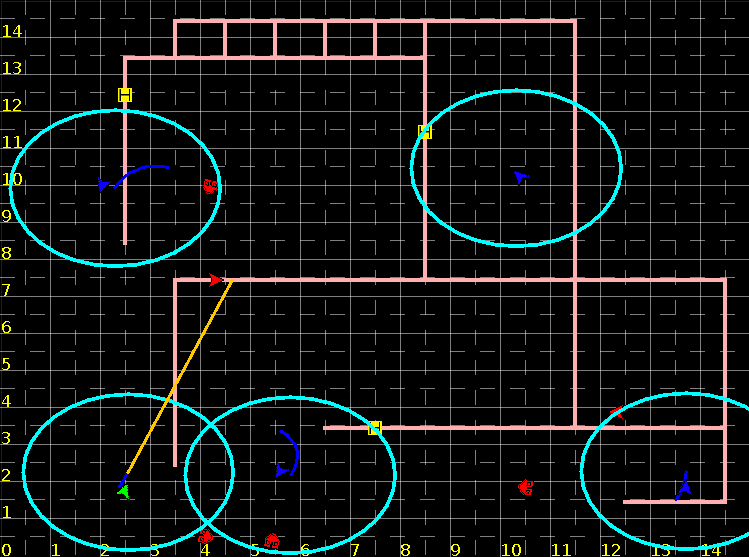
\includegraphics[scale=0.3]{comm_ranges.png}
	\caption{UAV communication ranges at $10\%$}
	\label{fig:comm_ranges}
\end{figure}

Each cell in the world grid is identified by a row and column index.  Each cell contains a probability of being empty, $P(empty)$, and a timestamp of when this data was last updated.  This is commonly called a Grid Based Occupancy Map. The probability value is updated in a Bayesian fashion by sensor scans during each time step of the simulation similar to~\cite{waharte}.  

The Bayesian Inference update equation is shown in equations~\ref{eq:bayesianEmptyDenom} and \ref{eq:bayesianEmpty} where $P_{t}(T_{i})$ is the current probability at time $t$ that a target $T$ of the $ith$ target type is present and  $P_{t-1}(T_{i})$ is the previous timestep's probability that a target $T$ of the $ith$ target type is present.  These values are taken from the Target Belief models described in the next section.  If no Target Belief is located in the cell being updated then these probabilities are set to zero.  $P(S_{i}|T_{i})$ is the probability of a sensor $S$ detecting target type $i$ and correctly perceiving it as a type $i$.  

Note in equation~\ref{eq:bayesianEmptyDenom} that the reverse of $P(S_{i}|T_{i})$ is used by subtracting it from $1$.  This is because we need the probability that the sensor missed detecting the target given that the target was actually present.  

\begin{equation}
\label{eq:bayesianEmptyDenom}
%P(miss) = \prod_{j=0}^{\text{All Target Types}} (1 - P(S_{j}|T_{j})) * P_{t-1}(T_{j})
P(miss) = \sum_{i=0}^{\text{All Target Types}} (1 - P(S_{i}|T_{i})) * P_{t-1}(T_{i})
\end{equation}

\begin{equation}
\label{eq:bayesianEmpty}
P_{t}(empty) = \frac{P(S_{e}|T_{e})*P_{t-1}(empty)}{ P(S_{e}|T_{e})*P_{t-1}(empty) + P(miss)}
\end{equation}

The $P(empty)$ probability is then used to derive a Discrete Shannon Uncertainty value as described in \cite{shannon} (also known as Shannon Entropy).  A Shannon Uncertainty curve is zero when $P(empty)$ is 0\% or 100\% since in those edges cases we know for certain if the cell is empty or not.  Conversely a Shannon Uncertainty curve is at its peak when we know nothing for certain when $P(empty)$ is 50\%.  Nominally a Shannon Uncertainty curve varies from zero to one when $P(empty) = 0.5$. The equation can be see in~\ref{eq:shannon} and is plotted in figure~\ref{fig:shannon}.

\end{multicols*}

\begin{equation}
\label{eq:shannon}
U = -P(empty) * \log_{2}(P(empty)) - ( 1-P(empty) * \log_{2}(1-P(empty)))
\end{equation}

\begin{multicols*}{2}
	
	\begin{figure}[H]
		\centering
		%\includegraphics[width=\linewidth,height=\textheight]{imagefile}
		\includegraphics[scale=0.4]{shannon.png}
		\caption{Shannon Uncertainty}
		\label{fig:shannon}
	\end{figure}
	
The goal of the mission is to find all of the targets and destroy them.  In order to guarantee that all targets have been found the UAVs must reduce the Shannon Uncertainty of each world cell to 0 in their shared belief model.  In practice the world cells are never all driven to 0 at once.  There is a global certainty decay rate that is applied to the cell beliefs at every time step.  It slowly drives $P(empty)$ back to 50\% over time.  This models the fact that unless a UAV is watching a cell they cannot know with 100\% certainty what is going on within that cell.  There is a chance that a moving target that has somehow evaded detection could be occupying a previously scanned world cell location.  So instead of requiring the uncertainty of all world cells to be at 0\% to end the mission we only require that all cells be driven below a user defined threshold percentage.

A more accurate dispersion of uncertainty would require all UAVs in the swarm to understand the kinematic limits of every target type in the mission area.  Upon detection and subsequent sensor loss of a mobile target, uncertainty should radiate outward from the target's last known location.  The rate and directionality of uncertainty propagation would be computed using the known maximum speed and turning characteristics of the target's suspected type. This more accurate technique was not utilized in this model because of the target data requirements.  Collecting and formatting this information for all of the pre-existing legacy vehicles in the swarm would be an additional burden on software retrofitting tasks.  It also poses additional intelligence gathering requirements before every deployment of the swarm.


%\section{Target Beliefs}
\subsection{Target Beliefs}
When a UAV detects something that might be a target it adds a Target Belief to its Belief Model.  The Target Belief contains an estimation of the target's location and orientation.  It also contains a list of all possible target types and an associated probability that the detected target is the corresponding type of target. The list of target type probabilities within a Target Belief always sum up to one.  At initialization all target types are equally likely.  As time progresses and more sensor detection attempts of the target are completed the probabilities per target type will converge to a single type.  As with Cell Beliefs the probabilities for target type's are updated using a Bayesian Inference system.  

The Bayesian Inference update equation for Target Beliefs is shown in equation~\ref{eq:bayesianTgt}.  The parameters in equation~\ref{eq:bayesianTgt} are the same as for Cell Beliefs with the addition of $P(S_{j}|T_{i})$ which is the probability of mis-perceiving a detection of a target type $i$ as a target type $j$.  This equation is applied for every suspected target type returned from a sensor scan of a world cell. After all of the sensor's possible target type results have been evaluated then the probabilities for all target types are normalized in the Target Belief such that equation~\ref{eq:probsNormalize} holds true.  The values for $P(S_{x}|T_{x})$ used in this work are listed in table~\ref{tab:snsrTgtProb}. \textbf{TODO: Heading estimate/update}

%is the Detected Target Type from a sensor scan and $TT$ is a Target Type. $P_{TT}(x)$ is the probability that the scanned target's type is the $x$ type.  This equation is applied for every suspected target type returned from a sensor scan.  After all of the sensor's possible target type results have been evaluated then the probabilities for all target types are normalized in the Target Belief.\textbf{TODO: mulitcol format}

%	P(\text{Detected Target Type} Y) = \frac{P(detect tgt type y) * P(prev belieft tgt Y exists)}{\sum_{T_{0}}^{Num Tgts}P(detect X as Y) * P(Prev beleif of X)}
%	P(\text{Target is detected type}) = \frac{P(\text{Detecting Target Type}) * P(\text{Previous Target is detected type})}{\sum_{i=T_{0}}^{All types}d}

%P(\text{(Mis)Classifying T_{i} as detected type}) * P(\text{Previous Target is T_{i}})

%\end{multicols*}

%\begin{equation}
%\label{eq:bayesian_verbal}
%P_{TT}^{'}(DTT) = \frac{ P(\text{Detecting }TT) * P_{TT}(DTT)} {\sum_{i=0}^{\text{Target types}}P(\text{ (Mis)Classifying } i \text{ as } DTT) * P_{TT}(i)}
%\end{equation}

\begin{equation}
\label{eq:bayesianTgt}
P_{t}(T_{i}) = \frac{P(S_{i}|T_{i})*P_{t-1}(T_{i})}{ \sum_{j=0}^{\text{All Target Types}}P(S_{j}|T_{i}) * P_{t-1}(T_{j}) }
\end{equation}

\begin{equation}
\label{eq:probsNormalize}
\left( \sum_{j=0}^{\text{All Target Types}}P_{t}(T_{j})\right)  = 1
\end{equation}

%	P_{TT}(DTT) = \frac{ P(\text{Detecting }TT) * P_{TT}(DTT)}  {ddd}


%\begin{multicols*}{2}
In addition to estimated data about the actual target, Target Beliefs encapsulate information about the tasks performed on the target.  This tasking data is collectively called the Target Task Status.  This data is used for coordinating activities within the swarm.  Since the swarm of UAVs has no centralized control system to allocate task assignments this process must be done by mutual consent within the swarm.  Each Target Belief has a Target Task Status that denotes who is performing tasks on a target and if the task is still eligible for others to take over.  The Target Task Status includes the following attributes.

\begin{description}
	\item [Monitor UAV ID] The ID of the UAV who has the best monitor score.
	\item [Monitor UAV Score] The best known score for monitoring the target.
	\item [Monitor Task State] An enumeration describing the current phase of task coordination for monitoring.
	\item [Monitor Update Timestamp] The time when the monitor data was last updated.
	\item [Attack UAV ID] The ID of the UAV who has the best attack score.
	\item [Attack UAV Score] The best known score for attacking the target.
	\item [Attack Task State] An enumeration describing the current phase of task coordination for the attack.
	\item [Attack Update Timestamp] The time when the attack data was last updated.
	\item [Target Destroyed Flag] A flag indicating if the target has been destroyed or not.
\end{description}

The Task State enumerations control when and who may bid on tasks.  There are subtle differences in their uses between the monitor tasks and the attack tasks.  These are explained in detail in  section~\ref{sec:uncoordTaskingMyWork}.

\textbf{TODO: Task state should be before Target Task Status so it's defined ahead of time.}

\begin{description}
	\item [NO TASK] This is the initial null condition given to the monitor and attack tasks.  In the monitor case it means the target was just discovered and no one has had a chance to process it.  In the attack case it means no one has confirmed that the target should be destroyed.
	\item [Open] The task is open to any and all bids.  No one has attempted to claim the task yet.
	\item [Enroute] This means the UAV with the corresponding ID is on its way to the target to perform the corresponding task.  Anyone else could overrule if they have better score than current best UAV.
	\item [Performing] The UAV with the corresponding ID is now performing the action.  No one else may overrule or otherwise subsume the action without a special exemption.%regardless of their score.
	\item [Complete] The task has been completed by the UAV with the corresponding ID.  In the monitor case the target has been confirmed as destroyed.  In the attack case a weapon has been deployed but the target is not necessarily destroyed.
\end{description}

%\section{Merging Beliefs}
\subsection{Merging Beliefs}
\label{sec:mergingBeliefs}
Each UAV in the swarm periodically broadcasts its internal Belief Model.  The model is shown in Object Diagram format in figure~\ref{fig:belief_object}.  The entire model is encoded and transmitted to all other swarm members within communications range.   When a UAV receives another swarm member's belief model it must be merged with the receiver's internal belief.  No UAV completely trusts any other UAV in the swarm.  All data is merged in a weighted or filtered fashion.  No data is copied 100\% as-is since there are no guarantees that any one UAV is perfectly correct about anything.  The merging process in this work is an implementation of the Fusion Update technique described in~\cite{shem} for merging multiple values of uncertainty.

\textbf{TODO: Multicol formatting issue}
%The entirety of the Belief Model is shown in figure~\ref{fig:belief_object} in an Object Diagram.
\end{multicols*}
\begin{figure}[H]
	\centering
	%\includegraphics[width=\linewidth,height=\textheight]{imagefile}
	\includegraphics[scale=0.75]{belief_object.png}
	\caption{Belief Model Object Diagram}
	\label{fig:belief_object}
\end{figure}
\begin{multicols*}{2}
	
%\textbf{TODO: Future work: Sensor type expertise should weigh into this}.

Merging Cell Beliefs is a simple process and is described in algorithm~\ref{alg:mergeCell} in section~\ref{sec:algorithms}.   In short the receiving UAV compares every single world cell with its counterpart in the sending UAV's data.  If the last update timestamp of the incoming cell data is more recent than the currently stored data then the cell data is merged.  The merge process is a weighted average.  When the merge occurs the receiving UAV's timestamp is set to the timestamp of sending UAV's data.  This prevents future belief broadcasts from the same sending UAV to trigger another re-merging of the exact same cell data.  This also prevents the same data from re-merging if a third party UAV forwards the belief data. 

Other alternative algorithms exist for for merging the belief data.  A Bayesian system is intractable because it would require every UAV in the swarm to know all of the characteristics of every other sensor in the swarm.  Every sensor detection would have to be encode in the belief data including all of the relative geometries between the sensor and target.  This would let the receivers recompute the entire world model with complete information.  The data transmission requirements and processing requirements for this merging system are enormous.  These requirements defeat the purpose of retrofitting legacy hardware platforms into a swarm but it would provide perfect synchronization between belief models.

Another alternative is to choose the belief data with the lower uncertainty.  The UAV with a lower uncertainty should have newer information, more sensor readings, or readings from better sensor(s).  If all of the sensors in the swarm had similar performance characteristics this would be a suitable method.  Problems arise when very poor sensors and very high quality sensors work together in the swarm.  No information about which sensor type performed a detection to update the belief model is encoded.  The belief model on the poor quality UAV may think it has very low certainty but in actuality it's just a collection of poor readings that are heavily mistaken.  The belief from a poor quality sensor might say that the $P(empty)$ of a cell is 10\% while the belief from a high quality sensor might say that the $P(empty)$ of that same cell is 90\%.  Both $P(empty)$ yield an uncertainty of roughly 0.4.  So which of these is the better one to choose in this case?  Without a better model of uncertainty that can account for these quality discrepancies this is not a viable alternative.

Using a weighted average is not a perfect solution but it is simple, intuitive, and easy to derive when comparing sensor and target type pairings.  It also prevents each UAV from having to know the details about every other UAV or sensor in the swarm.  The only one who knows all of the capabilities of the swarm is the human operator. It puts the responsibility on the swarm operator to give a relative strength per sensor and target type pairing.  It lets the operator set whether the UAV is extremely trusting of external data about a target (because the UAV has poor sensors about a target type) or distrustful of external data about a target (because the UAV has high quality sensors about the target type).

Table~\ref{tab:exampleCellMerge} shows an example of merging a single cell.  At some time in the simulation UAV 1 believes cell $[2, 6]$ has a 20\% of being empty (or in other words an 80\% chance that something is there). This probability was last updated at time 1234.  UAV 1 has broadcasted this belief data and UAV 2 has received it.  UAV 2 believes there is a 50\% chance that the same cell is empty but this data was last updated a long time ago at time 22.  Therefore UAV 2 will merge UAV 1's data for this cell.  Since alpha is set to 0.6 the new $P_{2,6}(empty)$ for UAV 2 is $0.6*(0.2) + (1-0.6)*(0.5)=0.32$.  After the merging is complete UAV 2's $P(empty)$ value is set to $0.32$ and the last update timestamp is set to UAV 1's timestamp.

\begin{table}[H]
	\caption{Example cell merging with $alpha=0.6$}
	\centering
	\rowcolors{1}{lightgray}{white}
	\label{tab:exampleCellMerge}
	\begin{tabular}{|r|c|c||c|c|}
		\hline
		& \multicolumn{2}{c||}{Before Merge} & \multicolumn{2}{c|}{After Merge} \\
		\hline
		UAV             & 1   & 2                            & 1   & 2 \\
		\hline
		$P_{2,6}(empty)$& 0.2 & 0.5                          & 0.2 & 0.32 \\
		\hline
		Timestamp       & 1234& 22                           & 1234& 1234 \\
		\hline
	\end{tabular}
\end{table}

Merging Target Beliefs is more complicated but uses a similar weighted averaging technique as merging Cell Beliefs.  The model in this paper assumes that the UAVs are able to perform target track fusion (also known has cross-track correlation) amongst themselves and assign each track a unique ID such as in~\cite{stroupe}, \cite{barooah}, and~\cite{spillings}.  This process is outside the scope of this paper.

As stated earlier Target Beliefs have an estimated location, orientation, and list of target type probabilities.  Now we assume they also have a unique identifier assigned by the target track fusion process.  This unique identifier is used as a first pass comparison filter when merging Target Belief data.  If the receiving UAV does not have any data for the incoming Target Belief it simply copies it verbatim.  If the receiving UAV already has data for the Target Belief then a more detailed inspection is required.  Target Beliefs only get merged if the received data is newer than the currently stored data.  In this case the estimated target orientation, position, and list of type probabilities are all averaged with a user defined weighting against the incoming data.  The formal algorithm is defined in algorithm~\ref{alg:mergeTarget}.

The Target Task Status within a Target Belief is also merged with incoming data.  Instead of performing weighted averages logic must be applied to determine if the task status data is still live and active or if the data is transmitted for historical reference only.  The formal algorithm is defined in algorithm~\ref{alg:mergeTaskStatus} of section~\ref{sec:algorithms}.
